\documentclass[letterpaper, 12pt]{thesisECFM}
\usepackage{macros}

%%	NO OLVIDE INCLUIR FUENTE DE LAS TABLAS Y FIGURAS

% Decomentar para anular recuadros en los hiperenlaces dentro del pdf
% \hypersetup{pdfborder={0 0 0}}

% Teoremas ---------------------------------------------------------
% estos ambientes son para teoremas, lemas, corolarios, otros
% si no los utiliza los puede obviar en su trabajo de graduación
\theoremstyle{plain}
\newtheorem{thm}{Teorema}[section]
\newtheorem{cor}{Corolario}[chapter]
\newtheorem{lem}{Lema}[chapter]
\newtheorem{prp}{Proposición}[chapter]

\theoremstyle{definition}
\newtheorem{exa}{Ejemplo}[chapter]
\newtheorem{defn}{Definición}[chapter]
\newtheorem{axm}{Axioma}[chapter]

\theoremstyle{remark}
\newtheorem{rem}{Nota}[chapter]

% Operadores y funciones -------------------------------------------
% Los siguientes son ejemplos de comandos definidos por el usuario
% puede borrarlos, únicamente están para mostrar cómo se construyen con LaTeX
\DeclareMathOperator{\Supp}{Supp}       \DeclareMathOperator{\vol}{Vol}%
\DeclareMathOperator{\Rz}{Re}           \DeclareMathOperator{\Iz}{Im}%

\newcommand{\R}{\mathbb{R}}             \newcommand{\Z}{\mathbb{Z}}%
\newcommand{\C}{\mathbb{C}}             \newcommand{\K}{\mathbb{K}}%
\newcommand{\N}{\mathbb{N}}             \newcommand{\Q}{\mathbb{Q}}%
\newcommand{\Af}{\mathfrak{A}}          \newcommand{\Bf}{\mathfrak{B}}%
\newcommand{\Cf}{\mathfrak{C}}          \newcommand{\Df}{\mathfrak{D}}%
\newcommand{\Ff}{\mathfrak{F}}          \newcommand{\Lf}{\mathfrak{L}}%
\newcommand{\Mf}{\mathfrak{M}}          \newcommand{\Sf}{\mathfrak{S}}%
\newcommand{\Hi}{\mathcal{H}}           \newcommand{\Ba}{\mathcal{B}}%
\newcommand{\nada}{\varnothing}         \newcommand{\To}{\longrightarrow}%
\newcommand{\RR}{[-\infty,+\infty]}     \newcommand{\df}{:=}%
\newcommand{\sani}{$\sigma$\nobreakdash-anillo}
\newcommand{\salg}{$\sigma$\nobreakdash-álgebra}
\newcommand{\ff}{f^{-1}}

\newcommand{\norm}[1]{\left\Vert#1\right\Vert}
\newcommand{\pnorm}[2]{\norm{#1}_{#2}}
\newcommand{\abs}[1]{\left\vert#1\right\vert}
\newcommand{\su}[2]{\left\{#1_{#2}\right\}}
\newcommand{\Su}[4]{\suce #1#2 _{#2=#3}^{#4}}
\newcommand{\union}[4]{\bigcup_{{#2}={#3}}^{#4} #1_{#2}}
\newcommand{\Union}[4]{\bigcup \limits_{{#2}={#3}}^{#4} #1_{#2}}
\newcommand{\inter}[4]{\bigcap_{{#2}={#3}}^{#4} #1_{#2}}
\newcommand{\Inter}[4]{\bigcap \limits_{{#2}={#3}}^{#4} #1_{#2}}

\newcommand{\pdual}[2]{\left<#1,#2\right>}
\newcommand{\bra}[1]{\left<#1\right\vert}
\newcommand{\ket}[1]{\left\vert#1\right>}
\newcommand{\braket}[2]{\left<#1\vert#2\right>}
\newcommand{\Braket}[2]{\left\vert#1\right>\! \left<#2\right\vert}
%%%%%%%%%%%%%%%%%%%%%%%%%%%%%%%%%%%%%%%%%%%%%%%%%%%%%%%%%%%%%%%%%%%%


% Cuerpo de la tesis -----------------------------------------------

\begin{document}

%% Datos generales del trabajo de graduación
\datosThesis%
{2}%						% física 1; matemática 2
{El módelo del árbol binomial aplicado en las finanzas}%		% Título del trabajo de graduación
{Javier de San José Recinos Ortega}%			% autor
{Phd. Ricardo Pontaza}%			% asesor
{1}		% mes y año de la orden de impresión
{2}							% femenino 1; masculino 2

%% Datos generales del examen general privado
\examenPrivado%
{M.Sc. Edgar Anibal Cifuentes Anléu}%	% director ECFM
{Ing. José Rodolfo Samayoa Dardón}%		% secretario académico
{Perengano}%		% examinador 1
{Zutano}%		% examinador 2
{Fulano 2}%		% examinador 3

{\onehalfspacing	% interlineado 1 1/2

\OrdenImpresion{ordenImpresion}		% incluye orden de impresión, guardada en pdf

\Agrade{agradecimientos}			% Agradecimientos

\Dedica{dedicatoria}				% Dedicatoria

\par}
 
\frontmatter    % --------------------------------------------------  Hojas preliminares

{\onehalfspacing	% interlineado 1 1/2

\tableofcontents    % Índice general vinculado

%%% \figurasYtablas{ lista_figuras }{ lista_tablas }; con valor 1 se incluye la lista,
%%% cualquier otro valor no la genera
\figurasYtablas{1}{1}

%%% INCLUYA LA SIMBOLOGÍA NECESARIA EN ESTE APARTADO
%%% NO CAMBIAR LA DEFINICIÓN DE LA TABLA LARGA


\chapter{LISTA DE SÍMBOLOS}

\begin{longtable}{@{}l@{\extracolsep{\fill}} p{4.75in} @{}}  %%%	NO CAMBIAR ESTA LÍNEA
  \textsf{Símbolo} & \textsf{Significado}\\[12pt]
  \endhead
  $:=$ & es definido por\\
  $\cong$ & es isomorfo a\\
  $\Leftrightarrow$ & si y sólo si\\
  $\varnothing$ & conjunto vacío\\
  $E^c$ & complemento de $E$\\
  $\varsubsetneq$ & estrictamente contenido\\
  $E\setminus F$ & diferencia entre $E$ y $F$\\
  $E\Delta F$ & diferencia simétrica entre $E$ y
  $F$\\
  $\mathcal{P} (X)$ & conjunto potencia de $X$\\
  $\chi_E$ & función característica de $E$\\
  $E_n\!\!\uparrow$ & $E_n$ es una sucesión
  creciente\\
  $\mathfrak{L}$ & \salg{} de los conjuntos
  Lebesgue"=medibles\\
  $\mathscr{S}$ & espacio muestral\\
  $\mathfrak{A}$ & \salg{} de eventos\\
  $(\mathscr{S},\mathfrak{A},P)$ & espacio de
  probabilidad\\
  $\mathscr{D}$ & espacio de las funciones de
  prueba\\
  $\mathscr{D}'$ & espacio de las distribuciones\\
  $\delta_0$ & medida de Dirac, función $\delta$ de Dirac o
  $\delta$-función\\
  $\Phi^{\times}$ & espacio antidual de $\Phi$\\
  $\Phi\subset \mathcal{H}\subset \Phi^{\times}$ &
  espacio de Hilbert equipado o tripleta de Gel'fand\\
  $\left\vert \psi \right>$ & vector \emph{ket}\\
  $\left< \psi \right\vert$ & funcional \emph{bra}\\
  $\left< \varphi \vert \psi \right>$ & \emph{braket}
\end{longtable}
  % Lista de símbolos

%%% Haga el diseño que más le guste
\chapter{OBJETIVOS}

\section*{General}
Escriba el objetivo general.


\section*{Específicos}
Enumere los objetivos específicos.
\begin{enumerate}
\item 
\item 
\end{enumerate}

      % Resumen y objetivos

%%% Haga el diseño que más le guste
\chapter{INTRODUCCIÓN}


      % Introducción

\mainmatter     % --------------------------------------------------  Cuerpo del Trabajo de Graduación
\chapter{CONCEPTOS PRELIMINARES}

% ---------------> conjuntos, funciones y sucesiones
\section{Conjuntos, funciones y sucesiones}

En adición a los conjuntos de puntos que se trabajan con normalidad
en Matemáticas ~---puras y aplicadas---, se tendrá que hacer uso
frecuentemente de los conjuntos de conjuntos, si por ejemplo $X$ es
la recta real, como un intervalo es un conjunto de puntos, es decir
un subconjuto de $X$, se tendrá que el conjunto de todos los
intervalos es un conjunto de conjuntos.

En especial, cuando una clase hace referencia a subconjuntos del
conjunto $X$, la llamaremos \textbf{familia}. En especial el
\textbf{conjunto potencia} $\mathcal{P} (X)=\{A\mid A\subseteq X\}$
es una familia de $X$. Asimismo, se definirá el \textbf{complemento}
de $A$ por \[A^c=\{x\mid x\notin A\}.\]

\begin{defn}\label{dfcp28} Una \textbf{función de selección}
para un conjunto $X$ es una función $f$ la cual asocia a cada
subconjunto no vacío $E$ de $X$ un elemento de $E$: $f(E)\in E$.
\end{defn}

\begin{axm}[de selección]\label{choice} Para cualquier conjunto
existe una función de selección.
\end{axm}

\begin{rem} Con frecuencia el axioma~\ref{choice} se presenta en
la forma: para cada $E\in \mathcal{P}(X)\setminus\{\nada\}$,
elegimos un elemento $x\in E$. Asimismo, es equivalente al lema de
Zorn, para más detalles consultar
~\cite[p. 97]{Halmo},~\cite[p. 338]{Haus} o~\cite[p. 14]{Hewit}.
\end{rem}

Una \textbf{clase disjunta} es una clase {\boldmath $A$} de
conjuntos tal que para cualquier par de conjuntos distintos de
{\boldmath $A$} son disjuntos, en este caso nos referiremos a la
unión de conjuntos de {\boldmath $A$} como \textbf{unión disjunta}.

Si $E$ es un subconjunto de $X$, la función $\chi _E$ definida para
$x\in X$ por la relación:
\begin{equation}\label{eq0}
    \chi_E(x)= \begin{cases}
    1, & \mbox{si } x\in E, \\
    0, & \mbox{si } x\notin E.
    \end{cases}
\end{equation}Es llamada \textbf{función característica}
del conjunto $E$. La correspondencia entre los conjuntos y sus
funciones características es inyectiva, y todas las propiedades de
conjuntos y operaciones entre conjuntos pueden ser expresadas por
medio de funciones características. 

%%%	TABLA CORTA, ÚNICAMENTE LLEVA LÍNEAS HORIZONTALES PARA SEPARAR BLOQUES

\begin{table}[ht]
\caption[título optativo de la tabla]{Propiedades de los espacios $L^p$. Fuente: tomada de \cite[Cap. 3]{Brez}.}\label{tablaLp}
\centering
\begin{tabular}{cccc}
\hline
Espacio & Reflexivo\footnote{En el sentido topológico.} & Separable & Dual \\ \hline %\hline
$L^p$, $1<p<\infty$  & Si & Si & $L^q$, $1/p+1/q=1$ \\
$L^1$ & No & Si & $L^\infty$ \\
$L^\infty$ & No & No & $L^1 \varsubsetneq (L^\infty)’$ \\ \hline
\end{tabular}
\end{table}\footnotetext{En el sentido topológico.} 

\begin{defn}\label{dfcp1}Si $\su En$ es una sucesión de
conjuntos, definiremos los conjuntos $\overline{\lim } E_n$ y
$\underline{\lim } E_n$ de la siguiente forma:
\[\begin{array}{cc}
  \overline{\lim} E_n=\limsup \limits_{n\rightarrow \infty}E_n =
  \bigcap \limits_{n=1}^\infty \Union Ein \infty ,&
  \underline{\lim} E_n=\liminf \limits_{n\rightarrow \infty}E_n =
  \bigcup \limits_{n=1}^\infty \Inter Ein \infty \\
\end{array}\] y los llamaremos \textbf{límite superior} y
\textbf{límite inferior}, respectivamente, de la sucesión $\su En$.
Si tenemos $\overline{\lim} E_n = \underline{\lim} E_n$, usaremos la
notación $\lim_n E_n$ para este conjunto. Si la sucesión es tal que
$E_n\subset E_{n+1},\ n=1,2,\dots$ le llamaremos \textbf{creciente}
y se denotará por $E_n\!\!\uparrow$ y su límite será $\lim
\limits_{n\rightarrow \infty}E_n = \union En1 \infty$; si es tal que
$E_n\supset E_{n+1},\ n=1,2,\dots$ le llamaremos
\textbf{decreciente} y se denotará por $E_n\!\!\downarrow$ y su
límite será $\lim \limits_ {n\rightarrow \infty}E_n = \inter En1
\infty$. En ambos casos nos referiremos a ella como
\textbf{monótona}.\end{defn}


\begin{defn}\label{dfcp2}Sea $f$ una aplicación definida del conjunto
$X$ al conjunto $Y$, es decir $f:X\To Y$. Para cualquier subconjunto
$T\subseteq Y$, definimos la \textbf{imagen inversa} de $T$, bajo
$f$, denotada por $\ff (T)$, como sigue:
\[\ff (T)=\{s\in X\mid f(s)\in T\}.\]\end{defn} 

\begin{thm}\label{thcp1}Para la aplicación $\ff :{\cal{P}} (Y)
\To {\cal{P}} (X)$ se tienen las propiedades siguientes:
\begin{enumerate}
    \vspace{-6pt} \item $\ff(\bigcup_j T_j) = \bigcup_j
    \ff(T_j)$.
    \vspace{-6pt} \item $\ff(\bigcap_j T_j) = \bigcap_j
    \ff(T_j)$.
    \vspace{-6pt} \item Si $T_1\cap T_2=\nada$, entonces
    $\ff(T_1)\cap \ff(T_2) = \nada$.
    \vspace{-6pt} \item $\ff(T^c) = [\ff(T)]^c$.
    \vspace{-6pt} \item $\ff(\nada) = \nada$.
    \vspace{-6pt} \item $\ff(Y) = X$.
\end{enumerate}
\end{thm}


Las propiedades (1) y (3) del teorema~\ref{thcp1} establecen las
condiciones para la unión disjunta en una familia en $Y$. Sea ahora
$\Df$ una familia cualquiera de subconjuntos de $Y$, y definamos la
familia $\ff (\Df)$ de subconjuntos de $X$ como
sigue:\begin{equation}\label{eq1}
    \ff(\Df) = \{A\subseteq X \mid
A = \ff(T) \mbox{ para algún } T\in \Df\} = \{\ff(T) \mid T\in
\Df\}.
\end{equation}

El sistema de numeros reales extendido o \textbf{recta real
extendida} es el conjunto definido por $\RR\df\R \cup \{-\infty,
+\infty\}$, con la siguiente relación de orden: para $a\in \R$
tenemos $-\infty <a< +\infty$. La topología para este conjunto se
define por declarar como abiertos a los siguientes conjuntos:
$(a,b),\ [-\infty,b),\ (a,+\infty]$ y cualquier unión de conjuntos
de este tipo. Cuando se haga referencia a los \textbf{numeros reales
extendidos} o \textbf{valor real extendido}, se estará hablando de
los numeros reales y de los símbolos $\pm\infty$. Cuando trabajamos
con teoría de la integración, nos encontraremos con $\infty$, una
razón es que algunas veces trataremos de integrar sobre conjuntos de
medida infinita, este es caso de la recta real.

Por tal motivo, se hacen las siguientes definiciones para
facilitar su manejo: $a+\infty = \infty+a \df \infty$ si $0\leq a
\leq \infty$,~y
\begin{equation}\label{eq4}
    a\cdot \infty = \infty \cdot a
\df\begin{cases}
  \infty, & \mbox{si } 0 < a \leq \infty \\
  0, & \mbox{si } a = 0 \\
\end{cases}
\end{equation}las leyes de cancelación se tratan
así: $a+b = a+c\ \Rightarrow\ b=c\ $ y $a\cdot b =a\cdot c\
\Rightarrow\ b=c$ sólo cuando $0 < a < \infty$. 

\begin{defn}\label{dfcp3}Sea $\su aj$ una sucesión en la recta
real extendida, y sean $b_k = \sup\{a_k,a_{k+1},a_{k+2}\dots\},\
k=1,2,3,\dots$, y $\beta = \inf\{b_1,b_2,b_3,\dots\}$. Entonces
llamaremos a $\beta$ el \textbf{límite superior} de $\su aj$, y
escribiremos $\beta = \limsup \limits_{j\rightarrow \infty}(a_j)$.
El \textbf{límite inferior} se define análogamente, al intercambiar
$\sup$ e $\inf$ en las anteriores definiciones; notemos que \[\liminf
\limits_{j\rightarrow \infty}(a_j) = -\limsup \limits_{j\rightarrow
\infty}(-a_j).\] Si $\su aj$ converge, entonces tenemos $\liminf
\limits_{j\rightarrow \infty}(a_j) = \limsup \limits_{j\rightarrow
\infty}(a_j) = \lim \limits_{j\rightarrow
\infty}(a_j)$.\end{defn}

\begin{prp}\label{prcp1}Si $0\leq a_1\leq a_2\leq \cdots$,
$0\leq b_1\leq b_2\leq \cdots$, tales que $a_j \To a$ y $b_j \To
b$. Entonces $a_j b_j \To ab$.
\end{prp}

\begin{defn}\label{dfcp4}Supongamos que $\su fj$ es una sucesión de
funciones de valor real extendido en un conjunto $X$. Entonces
$\sup_j f_j$ y $\limsup \limits_{j\rightarrow \infty} f_j$ son las
funciones definidas en $X$ por:
\[\left(\sup_j f_j\right)(x)\df \sup_j(f_j(x)),\quad \left(\limsup
\limits_{j \rightarrow \infty} f_j\right)(x)\df \limsup \limits_{j
\rightarrow \infty}(f_j(x)).\] Si $f(x)=\lim \limits_{j \rightarrow
\infty} f_j(x)$, y asumimos que el límite existe para cualquier
$x\in X$, entonces llamaremos a $f$ el \textbf{límite puntual} de la
sucesión $\su fj$ y hablaremos de \textbf{convergencia puntual} en
este contexto.\end{defn}

\begin{figure}[ht]
\centering
\label{fig:analisisGraficoModelo3}
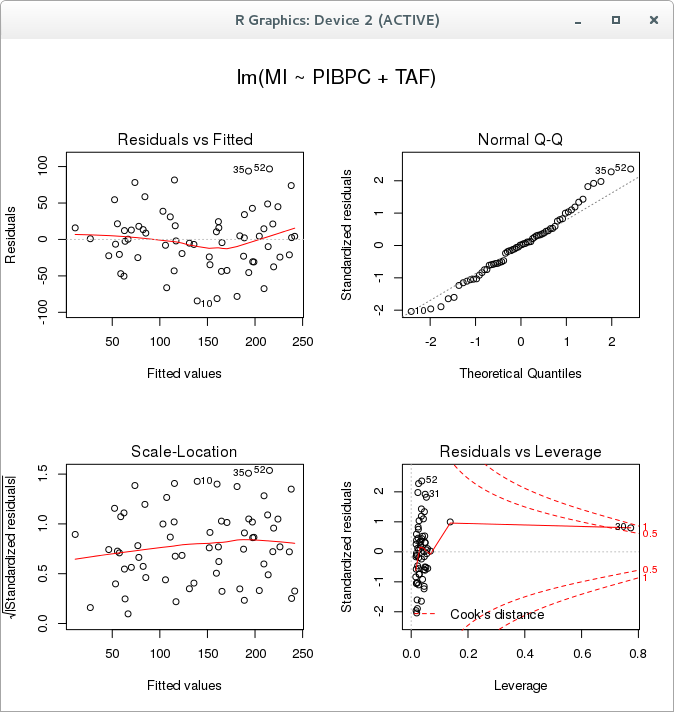
\includegraphics[width=0.9\linewidth]{analisisGraficoModelo3}\\
\caption[Titulo en el índice de figuras (opcional)]{Título en el 
documento. Las imágenes pueden ser raster (de preferencia jpg, png 
con buena resoloción para imprimir) o vectorial (convertir a pdf, en 
este caso la resolución no afecta) Fuente: imagen tomada de~\cite{liu}.}
\end{figure}


\begin{lem}\label{lmcp11}Sean $z,w \in \C$, $1 < p \leq 2$ y $1/p +
1/q = 1$. Entonces tenemos \[\abs{z+w}^q + \abs{z-w}^q \leq 2 (|z|^p
+ |w|^p)^{\frac{1}{p-1}}.\]
\end{lem}

\begin{proof} Consultar~\cite[p. 227]{Hewit}. \end{proof}

\begin{defn}\label{dfcp5}Sea $f:X\To \RR$ una aplicación. Se definen
las aplicaciones $f^+\!\df\max\{f,0\}$, $f^-\!\df-\min\{f,0\}$, a
$f^+$ y $f^-$ se les llama la \textbf{parte positiva y negativa} de
$f$, respectivamente.
\end{defn}


\begin{prp}\label{prcp2}Para cualquier aplicación $f:X\To \R$
denotaremos su valor absoluto con $\abs f$, entonces tenemos
\[\abs f=f^++f^-,\quad f=f^+-f^-.\]
\end{prp}

% --------------->  

\section{Tablas y Gráficas}

Las tablas y gráficas deben tener un título \verb|\caption{text}| que la identifique, debe especificar la \textbf{fuente}, y una etiqueta \verb|\label{text}| para hacer referencias cruzadas dentro del documento.

%% TABLAS LARGAS LLEVAN TODAS LAS DIVISIONES DE LOS BLOQUES

\begin{longtable}{|l|l|l|l|l|}
\caption[]{Diccionario de datos, tabla \textit{marn} (continuación)} \\ \hline

\multicolumn{1}{|c|}{\textbf{Name}} & \multicolumn{1}{c|}{\textbf{Data type}} & \multicolumn{1}{c|}{\textbf{Not Null?}} & \multicolumn{1}{c|}{\textbf{Primary key?}} & \multicolumn{1}{c|}{\textbf{Default}} \\ \hline \endhead
	\caption[Diccionario de datos, tabla \textit{marn}]{Diccionario de datos, tabla \textit{marn}. Fuente: obtenida de pgAdminIII}\label{data:marn} \\ \hline

	\multicolumn{1}{|c|}{\textbf{Name}} & \multicolumn{1}{c|}{\textbf{Data type}} & \multicolumn{1}{c|}{\textbf{Not Null?}} & \multicolumn{1}{c|}{\textbf{Primary key?}} & \multicolumn{1}{c|}{\textbf{Default}} \\ \hline \endfirsthead 

	id & \textit{integer} & \textit{Yes} & \textit{Yes} & \textit{nextval('marn\_id\_seq'} \\ %\hline

	 &  &  &  & \textit{::regclass)}\footnote{Note que la tabla es mas ancha que lo preestablecido. Procure diseñar elementos acordes con el espacio preestablecido.} \\ \hline

	\multicolumn{ 5}{|l|}{Clave primaria que  obtendrá su valor de forma secuencial al ingresar un nuevo registro} \\ \hline
		lista\_tax & \textit{text} & \textit{No} & \textit{No} & \textit{} \\ \hline

	\multicolumn{ 5}{|l|}{Clasificación del proyecto en base al Listado Taxativo del MARN} \\ \hline
		no\_marn & \textit{text} & \textit{No} & \textit{No} & \textit{} \\ \hline

	\multicolumn{ 5}{|l|}{Numero de expediente asignado por el MARN} \\ \hline
		date0 & \textit{date} & \textit{No} & \textit{No} & \textit{} \\ \hline

	\multicolumn{ 5}{|l|}{Día del ingreso del expediente del proyecto (instrumento ambiental) en el MARN} \\ \hline
		notas & \textit{text} & \textit{No} & \textit{No} & \textit{} \\ \hline

	\multicolumn{ 5}{|l|}{Observaciones} \\ \hline
		no\_res\_ap & \textit{text} & \textit{No} & \textit{No} & \textit{} \\ \hline

	\multicolumn{ 5}{|l|}{Numero de resolución aprobatoria del proyecto por el MARN%
	\footnote{Note que en esta línea la tabla se corta y continua en la siguiente página. 
	Utilizar paquete \textsf{longtable} y ambiente \textit{longtable}.}} \\ \hline
		date\_res\_ap & \textit{date} & \textit{No} & \textit{No} & \textit{} \\ \hline

	\multicolumn{ 5}{|l|}{Día de emisión de la resolución aprobatoria por el MARN} \\ \hline
		date0\_fianza & \textit{date} & \textit{No} & \textit{No} & \textit{} \\ \hline

	\multicolumn{ 5}{|l|}{Día de emisión de fianza del proyecto.} \\ \hline
		no\_res\_fianza & \textit{text} & \textit{No} & \textit{No} & \textit{} \\ \hline

	\multicolumn{ 5}{|l|}{Numero de la resolución de aceptación de fianza por el MARN} \\ \hline
		date1\_fianza & \textit{date} & \textit{No} & \textit{No} & \textit{} \\ \hline

	\multicolumn{ 5}{|l|}{Fecha de inicio de fianza} \\ \hline
		date2\_fianza & \textit{date} & \textit{No} & \textit{No} & \textit{} \\ \hline

	\multicolumn{ 5}{|l|}{Fecha de finalización de fianza (renovación)} \\ \hline
		lic\_ambiental & \textit{text} & \textit{No} & \textit{No} & \textit{} \\ \hline

	\multicolumn{ 5}{|l|}{Numero de licencia ambiental} \\ \hline
		date\_lic\_ambiental & \textit{date} & \textit{No} & \textit{No} & \textit{} \\ \hline

	\multicolumn{ 5}{|l|}{Fecha de finalización de ultima licencia ambiental} \\ \hline
		proyecto\_id & \textit{integer} & \textit{Yes} & \textit{No} & \textit{} \\ \hline

	\multicolumn{ 5}{|l|}{Enlace con la tabla proyecto\_id} \\ \hline
\end{longtable}




\chapter{Conceptos Financieros }
\section{Acciones,Opciones, Calls y Puts}
Una \textbf{acción} es un título emitido por una sociedad que representa el valor de las fracciones iguales en que se divide su capital social. Que además la empresa puede decidir ponerlas en venta a los inversores, en el cual tiene clasificaciones:
	\begin{itemize}
		\item Acciones de clase A 
		\item Acciones de clase B
	 
	\end{itemize}
 	
 		\textbf{ Acciones de clase A }: Son aquellas acciones en las cuales, uno puede ejercer dividendos\footnote{Es la parte del beneficio de una empresa que se reparte entre los accionistas de una sociedad.} y toma de decisiones de la empresa.
 		\newline
 		\textbf{ Acciones de clase B}: Son aquellas que no ejercen derechos de la empresa ni cobrar dividendos, solo son acciones con cierto valor, por lo general están cotizadas en una \textbf{bolsa de valores}\footnote{Es una organización privada que brinda las facilidades necesarias para que sus miembros, atendiendo los mandatos de sus clientes, como realizar venta y compra de valores, tales como bonos, acciones de sociedades.}.
 		\newline
 		Para las acciones de clase B las empresas utilizan esas inversiones para proyectos, ampliaciones, o cosas que necesiten la empresa; pero las empresas están obligadas a dar sus estados financieros, eso quiere decir que están obligados a presentar su contabilidad y sus ventas.  \newline
	Con la siguiente gráfica podemos apreciar como se comporta una acción de clase B, esta gráfica fue sacada de Yahoo finance en donde esta abierta para todo publico para cotizar acciones.
\begin{figure}[h]
	\centering
	\label{Accion de Google cotizadas en NASDAQ}
	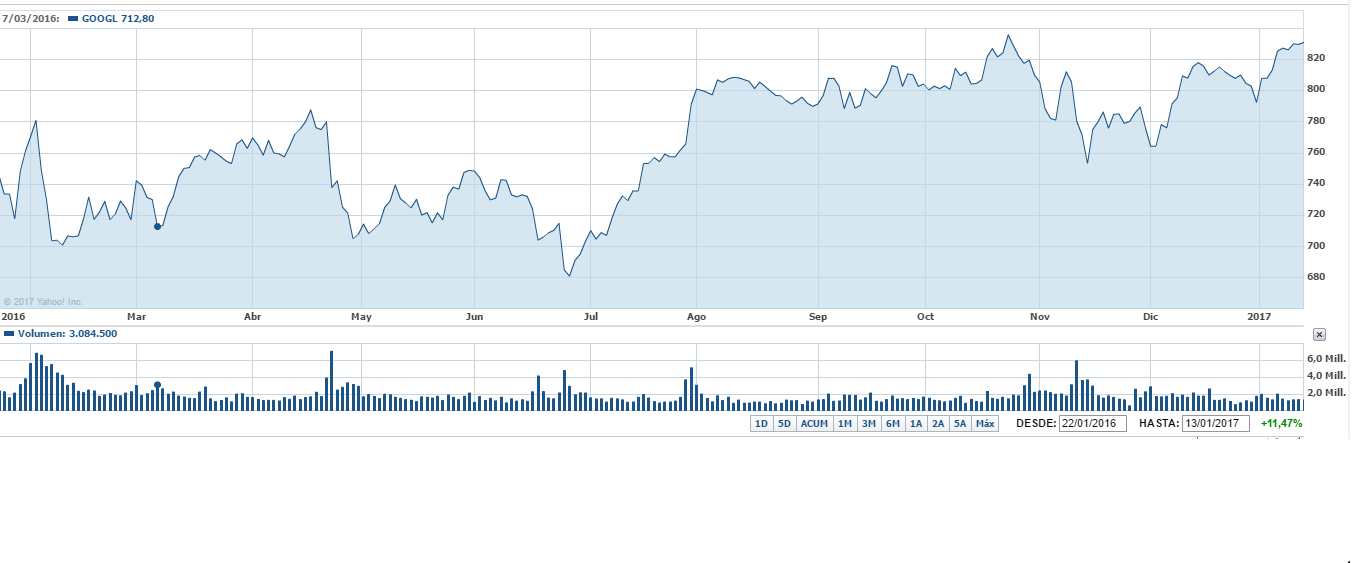
\includegraphics[width=1.2\linewidth]{google}\\
	\caption[Titulo en el índice de figuras (opcional)]{Acción de Google  cotizada en la bolsa de valores de U.S.A}
\end{figure}
		\newpage
		Como se puede apreciar en la gráfica ( él lado derecho) es el valor del precio de una acción en dolares, en la parte inferior tenemos el \textbf{volumen}\footnote{El volumen de una acción es el numero de transacciones. } de la acción.
		 \newline
		 las acciones se comportan de forma estocástica, dado que tienen un cierre y una apertura, por lo general una acción vista en forma diaria se aprecia como en la gráfica 1.
		  \newline
		 \begin{figure}[h!]
		 	\centering
		 	\label{Apertura y cierre}
		 	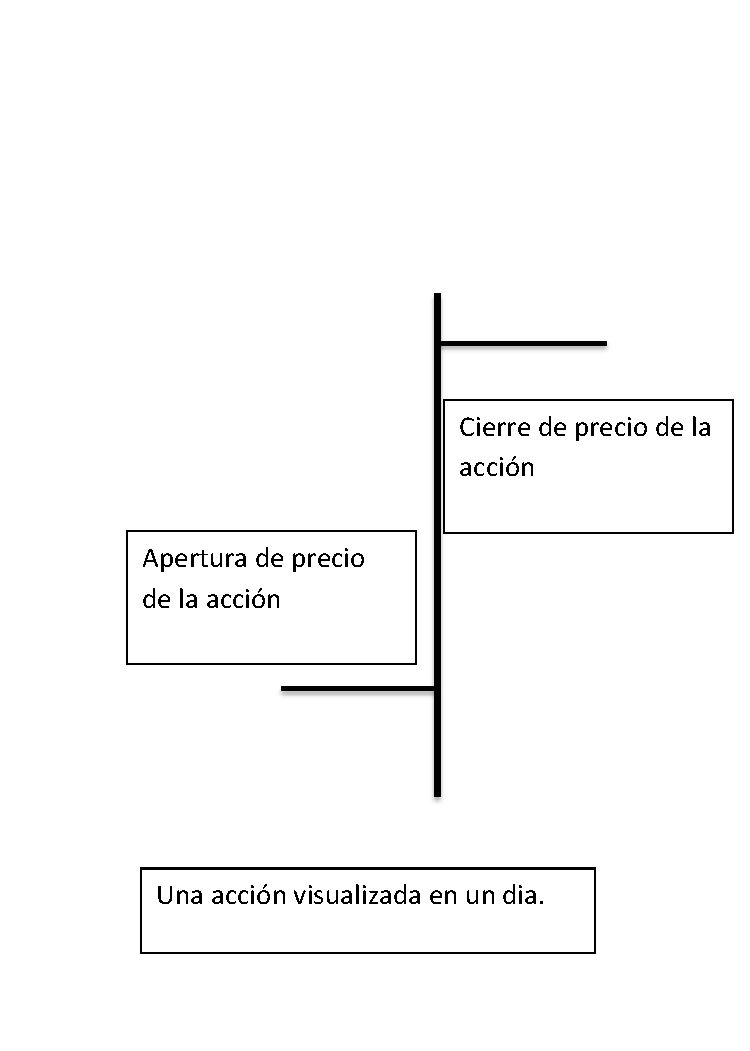
\includegraphics[width=0.35\linewidth]{a}\\
		 	\caption[Titulo en el índice de figuras (opcional)]{Comportamiento de una acción cuando el mercado esta abierto.}
		 \end{figure}
		  \newpage
Una \textbf{opción} es un contrato que se da a su comprador el derecho pero no la obligación a comprar o vender bienes, hasta una fecha concreta existen dos tipos de opciones:
	\begin{itemize}
		\item Opción de compra (Calls) 
		\item Opción de venta (Puts) 
	
	\end{itemize}

Un \textbf{call} es una opción de compra, en el que uno tiene el derecho pero no la obligación de comprar las acciones asociadas; si se emite un \textbf{Call} tiene la obligación de entregar las acciones asociadas al precio de ejecución.    	
		\newline
Un \textbf{Put} es una opción de venta, en el que uno tiene el derecho pero no la obligación de vender las acciones asociadas; si se emite un \textbf{Put} tiene la obligación de entregar las acciones asociadas al precio de ejecución.    	
\newline		
\begin{defn}Un \textbf{ Call} es $ C=Max(0,S-X) $;donde $ X $ es el precio de la opción y $ S $ es el precio de la acción.	
	\end{defn}
\begin{defn}Un \textbf{ Put} es $ C=Max(0,X-S) $;donde $ X $ es el precio de la opción y $ S $ es el precio de la acción.	
\end{defn}	
\subsection{Rentabilidad a lo largo}
Una rentabilidad a lo largo para un \textbf{call} es cuando la acción sube de precio entonces, el precio de la opción sube.	
\newline 
Aquí va una imagen
\newline 
Una rentabilidad a lo largo para un \textbf{put} es cuando la acción baja de precio entonces, el precio de la opcion sube.	
\newline 
Aquí va una imagen
\newline 
\subsection{Rentabilidad a lo corto}
Una rentabilidad a lo largo para un \textbf{call} es cuando la accion baja de precio entonces, el precio de la opcion naja.	
\newline 
Aqui va una imagen
\newline 
Una rentabilidad a lo corto para un \textbf{put} es cuando la accion sube de precio entonces, el precio de la opcion baja.	
\newline 
Aqui va una imagen
\section{Valor Intriseco}
Es cuando el valor del bien menos el derecho que vale, sus tres formas que se pueden dar son:
	\begin{itemize}
		\item In the Money
		\item At the Money 
		\item out of the Money
	
	\end{itemize}

Si es \textbf{In the Money} para un \textbf{call} es si el precio de ejecución de un call es mayor que el precio de la acción en pocas palabras $ S > X $.
\newline
Si es \textbf{In the Money} para un \textbf{put} es si el precio de ejecución de un put es menor que el precio de la accion en pocas palabras $ X > S $.
\newline
Si es \textbf{At the Money} para un \textbf{Call} es si el precio de ejecución de un call es igual que el precio de la accion en pocas palabras $ S = X $.
\newline
Si es \textbf{At the Money} para un \textbf{Put} es si el precio de ejecución de un put es igual que el precio de la accion en pocas palabras $ S = X $.
\newline
Si es \textbf{out the Money} para un \textbf{Call} es si el precio de ejecución de un call es menor que el precio de la accion en pocas palabras $ S < X $.
\newline
Si es \textbf{out the Money} para un \textbf{Put} es si el precio de ejecución de un put es mayor que el precio de la acción en pocas palabras $ X < S $.

\begin{defn}Una \textbf{ Prima de una opción} es el precio del contrato o de la opción en pocas palabras es: 
	\begin{equation}\label{eq1}
	Prima= V.I +V.T
	\end{equation}
	Donde $ V.I $ es el valor intrínseco y $ V.T $ es el valor del tiempo.
\newline
El \textbf{Valor del tiempo} de una opción se desvanece con mayor rapidez a partir de sus últimos días de expiran.
\section{Estrategias sobre opciones}
Las estrategias sobre opciones implican tomar posiciones en opciones, los activos subyacentes, y los prestamos otorgados, las 4 posiciones que tienen son: \textbf{call a lo largo, call a lo corto, put a lo largo y un put a lo corto}. Las estrategias pueden ser de tres tipos:
		\begin{itemize}
			\item Alcista
			\item Mercado pesimista 
			\item Neutral
			
		\end{itemize}
En términos de perspectivas del mercado pueden ser tres:\textbf{Agresivo, defensivo y Riesgos } el termino de riesgo viene por obtener beneficios en mercados calmados.		
	
			\section{Valor del dinero en el tiempo}
			El \textbf{interés} es el costo de pedir prestado dinero, entonces sea $ r $ el interés anual, si el interés es compuesto una vez por año , entonces el valor del futuro ($ VF $)	de una cantidad inicial  $ P $ después de n años es.
			\begin{equation}\label{eq0}
		    VF=P(1+r)^{n}
			\end{equation}
			el valor presente ($ VP $) que es el valor del día de hoy se puede escribir como:		
							\begin{equation}\label{eq0}
							P=VF(1+r)^{-n}
							\end{equation}
				\subsection	{Valor presente}
				Sea ($ VP $) y sea $ C_{n} $ un fluido de dinero a través del tiempo $ 1,2,\cdots,n $ y $ r $ el interés anual es:
						\begin{equation}\label{eq0}
						VP= \dfrac{C_{1}}{(1+r)}+\dfrac{C_{2}}{(1+r)^{2}}+\cdots+\dfrac{C_{n}}{(1+r)^{n}}
						\end{equation}	
				\section{Opciones arbitrarias}		
						Una oportunidad de arbitraje sin riesgo es aquella que, sin ninguna inversión inicial, genera una rentabilidad no negativa en todas las circunstancias y rendimientos positivos. En un mercado eficiente.
						\textbf{El principio dominante del portafolio} dice que él portafolio A debería ser mas valioso que el portafolio B si la rentabilidad de A es al menos tan buena bajo todas las circunstancia.\newline
						Derivando las relaciones libres de arbitraje que los valores de las opciones deben de satisfacer. Estas relaciones son independientes del modelo probabilístico del precio de acciones, solo asumimos que no hay costo de transacción y los prestamos están disponibles a la tasa de interés sin riesgo, las tasas de interés son no negativas y no hay oportunidad de arbitraje, simplificando esto tenemos que el tiempo sea cero. $ VP(x) $ donde $ x $ son los dolares a expirar. 
							\begin{equation}\label{eq0}
							VP(x)= xd(\tau) 
							\end{equation}
							
							Donde $ \tau $ es el tiempo a expirar
							\begin{lem}\label{lmcp11}
								En la bolsa americana un $ call $ y un $ put  $ con tiempo mas largo a la expiración no puede valer menos que un $ call $ y un $ put $ en un menor tiempo de expiración 
							\end{lem}
							
							\begin{lem}\label{lmcp11}
							La opción $ Call $ y $ put $ con un precio de ejercicio mas alto (mas bajo) respectivamente no puede valer mas que un $ call $ y un $ put $ idéntico con un precio de ejercicio mas bajo  (más alto).
							\end{lem}
							
							\begin{lem}\label{lmcp11}
							La diferencia en los valores de dos opciones por lo demás idénticas no puede ser mayor que la diferencia de sus precios de ejercicio
							\end{lem}
							
								\begin{proof} 
									Consideremos los Calls nada mas. Sea 2 precios de ejercicio tal que $ X_{1}<X_{2} $. Asumamos que $ C_{1} - C_{2}<X_{2}-X_{1} $ en lugar. Compramos el precio mas bajo $ C_{2} $ y escribimos a $ C_{1} $ el precio mas alto, generando retornos positivos y depositando $ X_{2}-X_{1} $ en una cuenta sin riesgo en un banco.
									  \newline
									  Supongamos que se ejecuta $ C_{1} $ antes del tiempo de expiracion, tendríamos dos casos. Si $ C_{2} >S-X_{1}$, entonces vendemos $ C_{2} $, la rentabilidad de la venta seria $ C_{2}-(S-X_{1})>0 $ de lo contrario $ C_{2} $ realizaría un flujo de caja de $ X_{1}-X_{2} < 0  $ , en ambos casos cerramos la transacción con el dinero en el banco realizaríamos un flujo de efectivo no negativo. \newline
									  Supongamos ahora que no se ejecuta antes de la fecha de vencimiento $ C_{1} $, entonces el flujo de efectivo es 0, $ X_{1}<S $ , y $ X_{1}-X_{2} < 0 $, respectivamente si $ S \leq X_{1} $, $ X_{1}<S<X_{2} $ y $ S\leq X_{2} $, el flujo sigue siendo no negativo despues de que el dinero se agrega en la cuenta bancaria. 
									   
								\end{proof}
								\subsection	{La paridad de una opción }
							Supongamos que la acción no paga dividendos en efectivo o que las opciones están protegidas para que los valores de las opciones sean insensibles a los dividendos en efectivo. Por lo tanto, los resultados de las opciones protegidas no se enumeran por separado.	\newline
							El principio del no arbitraje implica que la inversión inicial establece que el portafolio también debe de ser nula. Con esto tenemos la paridad para las opciones europeas:
							
							\begin{equation}\label{eq0}
							C=P+S-VP(x)
							\end{equation}
							Consideremos $ C-P= S-VP(x) $ lo que implica que un $ call  $ a lo largo y un $ put $ a lo corto ponen a una posición larga en acciones y toman prestado $ VP $ del precio de ejercicio en pocas palabras es tomar una acción a lo largo como comprar acciones en margen. entonces la paridad del call y del put seria:
								\begin{equation}\label{eq0}
								C=(S-X) + [X-VP(x)]+P \geq S-X
								\end{equation}
								Por que $ C\geq 0 $ dado que $ C\geq max (S-X) $, el valor intrínseco; un call americano no puede valer menos que su valor intrínseco. por lo tanto tenemos los siguientes lemas. 
								\begin{lem}\label{lmcp11}
									Un call de una acción que no paga dividendos nunca vale menos que su valor intrínseco 
									
								\end{lem}
									\begin{lem}\label{lmcp11}
									Para los put europeos, $ P\geq max(VP(X)-S,0) $ 	
									\end{lem}
									\begin{thm}
									Un Call americano se ejercerá solo al momento del vencimiento o justo antes de que se venza los dividendos
									
									\end{thm}
									\subsection	{Convexidad de los precios de la opciones }
										\begin{thm}
										 la convexidad de los precios de las opciones, tenemos que para tres calls con precio de ejercicio idénticos $ X_{1}<X_{2}<X_{3} $, tenemos el: 
											\newline
											$ C _{X_{2}} \leq \lambda C _{X_{1}} + (1-\lambda) C _{X_{3}} $ , $ P _{X_{2}} \leq \lambda P _{X_{1}} + (1-\lambda) P_{ X_{3}} $
											\newline
											Donde $ \lambda = (X_{3}-X_{2}/(X_{3}-X_{1})) $	
										\end{thm}
									\begin{proof} 
									Supongamos que no es convexa, primero anotamos en nuestro portafolio a $  C _{X_{2}}  $ entonces compramos $  \lambda C _{X_{1}}  $, y compramos $ (1- \lambda) C _{X_{3}}  $, estamos generando un flujo  efectivo positivo. si call a lo corto no es ejecutado antes del día de expiracion manteniendo los calls hasta la expiracion el flujo de caja es descrito como:\newpage
								
								
							\begin{longtable}{|l|l|l|l|l|}
									\hline 
									& $ S\leq X_{1} $ & $ X_{1}< S \leq X_{2} $  & $ X_{2}<S<X_{3} $  & $ X_{3}\leq S $  \\ 
									\hline 
									Call descrito en $ X_{2} $& 0  & 0  & $ X_{2}-S $ & $ X_{2}-S $  \\ 
									\hline 
									$ \lambda $ calls compradas en $ X_{1} $& 0  & $ \lambda (S-X_{1}) $ &$ \lambda (S-X_{1}) $  & $ \lambda (S-X_{1}) $  \\ 
									\hline 
									$1- \lambda $ calls compradas en $ X_{3} $& 0  & 0  & 0 & $(1- \lambda )(S-X_{3}) $   \\ 
									\hline 
									& 0 &$ \lambda (S-X_{1}) $  & $ \lambda (S-X_{1}) $ + ($ X_{2}-S $ )  & 0 \\ 
									\hline 
							\end{longtable}  
								 Tenemos que el flujo de dinero es 0 o positivo, esto es una propiedad de arbitraje.
								 \newline
								 Supongamos que el call a lo corto se ejerce anticipadamente cuando el precio de la acción $ S $. Si 	$  \lambda C _{X_{1}} + (1-\lambda) C _{X_{3}}> S-X_{2} $, vendemos calls a lo largo para generar un flujo de dinero de 	$  \lambda C _{X_{1}} + (1-\lambda) C _{X_{3}} - (S-X_{2})>0 $. De lo contrario, ejecute calls a lo largo y entregue las acciones, entonces el flujo neto de  dinero es $ -\lambda X_{1}- (1-\lambda)X_{3}+X_{2} = 0  $De nuevo tenemos que es una propiedad arbitraria. \newline
								 Por el lema 2.3, sabemos que la pendiente del valor de un call (put), cuando se traza con el precio de ejercicio, es a lo mas uno (menos uno, respectivamente). esto prueba que se forma la convexidad.
									 \end{proof}
									 
									 \section	{Conceptos de los modelos financieros }
									En esta parte solo sera una breve definición, y en el otro capítulo sera el contenido mas detallado.
									\subsection	{Árbol binomial}
									
									En el  modelo del Árbol binomial en opciones y en acciones, tenemos que el tiempo es discreto y una medida en periodos, el modelo asume que si el precio actual de la acción es$ S $, puede subir su precio $ Su $ con una probabilidad $ q $, ahora si el precio de la acción baja $ Sd $ tiene que tener una probabilidad de $ 1-q $, donde $ 0<q<1 $ y $ d<u $. En efecto, $ d<R<u $ donde $ R=e^{\widehat{r}} $ con $ \widehat{r} >0 $ , Resultando que se necesita 6 datos conocidos para determinar el valor de la opción basándose en las condiciones de arbitraje: $ S $, $ u $,$ d $,$ X $,$ \widehat{r} $ y el numero de periodo antes de la expiración.
									\newline
									Aqui va una imagen
									\subsection	{Simulación Monte Carlo}
									La simulación de Monte Carlo es una técnica que utiliza muestreo aleatorio para estimar los resultados del modelo. Las estadísticas calculadas sobre estos resultados, tales como media, desviación estándar y percentiles. Entonces el método de Monte Carlo se puede interpretar como el valor esperado de una variable aleatoria $ Z $ definida como  
										\begin{equation}\label{eq0}
										Z=\dfrac{max (0,Su^{j}d^{n-j} - X)}{R^{n}}
										\end{equation}
										Con probabilidad $ b (j;n,p) $ con $ 0\leq j\leq n	  $
										
											\subsection	{Black- Scholes}
											Es la formula matemática utilizada para obtener los precios de las opciones sobre divisas fijas, fecha caducidad, el modelo genera precios basado e un conjunto de ideales relacionados con la volatilidad, distribución normal y las densidades de probabilidad, los principales impulsadores del modelo de fijación de precios son el precio de divisas, valor intrínseco, el tiempo de caducidad y la volatilidad, el la formula de Black- Scholes esta dado como: 
												\begin{equation}\label{eq0}
												C=S N(x) - Xe^{-r\tau}N(x-\sigma\sqrt{\tau})
												\end{equation}
												y para Put
													\begin{equation}\label{eq0}
													P=Xe^{-r\tau} N(-x+\sigma\sqrt{\tau}) - SN(-x)
													\end{equation}
													Donde $ x=\dfrac{Ln(S/X)+(r+\frac{\sigma^{2}}{2})}{\sigma \sqrt{\tau}} $
													
													      % Cap. 1 

\include{tch2}      % Cap. 2 

\include{tch3}      % Cap. 3 

\backmatter     % --------------------------------------------------  Apartados finales

%%% INCLUYA SUS CONCLUSIONES Y RECOMENDACIONES


\chapter{CONCLUSIONES}
\begin{enumerate}
	\item Conclusión 1.
	\item Conclusión 2.
	\item Conclusión 3.
\end{enumerate}

\chapter{RECOMENDACIONES}
\begin{enumerate}
	\item Recomendación 1.
	\item Recomendación 2.
	\item Recomendación 3.
\end{enumerate}
     % Conclusiones y recomendaciones

\begin{thebibliography}{99}
%% La bibliografía se ordena en orden alfabético respecto al apellido del 
%% autor o autor principal
%% cada entrada tiene su formatado dependiendo si es libro, artículo,
%% tesis, contenido en la web, etc

% artículo en una revista arbitrada
\bibitem{albin} P. Albin, E. Leichtnam, R. Mazzeo y P. Piazza. The signature package on Witt spaces. \textit{Ann. Sci. Ec. Norm. Supér. (4)}, \textbf{45}(2):241--310, 2012.

% libro
\bibitem{Brez} H. Brezis. \textit{Analyse functionnelle, théorie et applications.} (Collection Mathématiques Appliquées pour la Maítrise) Masson, Paris, 1992.

% libro
\bibitem{Choq} Y. Choquet"=Bruhat y otros. \textit{Analysis, manifolds and physics. (volumen 1)} North"=Holland Publishing Company, Amsterdam, 1996.

% libro
\bibitem{C:H2} R. Courant y {D. Hilbert}. \textit{Methods of mathematical physics. (volumen 2)} Interscience Publishers, Nueva York, 1962.

% artículo en la web arXiv, preprint
\bibitem{Rafa4} R. {De la Madrid}. The rigged {Hilbert} space of the free hamiltonian. Consultado en marzo de 2005 en \burl{http://arxiv.org/abs/quant-ph/0210167}.

% libro con datos faltantes, s.e. "sin editorial"
\bibitem{Doc} J. Escamilla-Castillo. \textit{Topología.} 2"a ed. s.e., Guatemala, 1992.

% libro traducido
\bibitem{Hasr} N. Haaser y {J. Sullivan}. \textit{Análisis real.}  Tr.~Ricardo Vinós. Trillas, México, 1978.

% libro traducido
\bibitem{Halmo} P. Halmos. \textit{Teoría intuitiva de los conjuntos.} 8"a ed. Tr.~Antonio Martín. Compañía Editorial Continental, S.A., México, 1973.

% libro 
\bibitem{Haus} F. Hausdorff. \textit{Set theory.} 2"a ed. Chelsea Publishing Company, Nueva York, 1962.

% libro
\bibitem{Heis} W. Heisenberg. \textit{The physical principles of the quantum theory.} Dover Publications, Inc., Nueva York, 1949.

% libro
\bibitem{Hewit} E. Hewitt y {K. Stromberg}. \textit{Real and abstract analysis.} Springer"=Verlag, Nueva York, 1965.

% libro
\bibitem{Kolmo} A. Kolmogorov y {S. Fomin}. \textit{Elementos de la teoría de funciones y del análisis funcional.} Tr.~Carlos Vega. MIR, Moscú, 1975.

% artículo de una enciclopedia en línea
\bibitem{Kronz} F. Kronz. Quantum theory: von {Neumann} versus {Dirac}. Consultado en marzo de 2005 en \burl{http://plato.stanford.edu/entries/qt-nvd/}.

% artículo en una revista arbitrada
\bibitem{liu} K. Liu, X. Sun, and S.-T. Yau. Goodness of canonical metrics on the moduli space of Riemann surfaces. \textit{Pure Appl. Math. Q.}, \textbf{10}(2):223--243, 2014

% artículo en una revista arbitrada
\bibitem{leader} E. Leader and C. Lorcé, The angular momentum controversy: What's it all about and does it matter?, \textit{Phys. Rept.} \textbf{541}, 163 (2014).

% libro
\bibitem{Omnes} Omn\`{e}s, R. \textit{The interpretation of quantum mechanics.} (Princeton Series in Physics) Princeton University Press, Princeton, 1994.

% libro
\bibitem{Penr} R. Penrose. \textit{La mente nueva del emperador.} Tr.~José García. Fondo de Cultura Económica, México, 1996.

% publicación electrónica
\bibitem{Ster} S. Sternberg. Theory of functions of a real variable. Consultado en abril de 2005 en \burl{http://www.math.harvard.edu/\~shlomo}.

% publicación electrónica
\bibitem{Tesc} G. Teschl. Mathematical methods in quantum mechanics with applications to {Schrödinger} operators. Consultado en abril de 2005 en \burl{http://www.mat.univie.ac.at/\~gerald}.

\end{thebibliography}
   % Bibliografía

\par    }          % termina interlineado 1 1/2

\end{document}


